\section{Convolutional Neural Networks for Risso’s Dolphins Identification}

\begin{center}
    \author{
    Rosalia Maglietta,
    Vito Renò,
    Rocco Cacioppoli,
    Emanuele Seller,
    Stefano Bellomo,
    Francesca Cornelia Santacesaria,
    Roberto Colella,
    Giulia Cipriano,
    Ettore Stella,
    Karin Hartman,
    Carmelo Fanizza,
    Giovanni Dimauro,
    \emph{(Member, IEEE)},
    Roberto Carlucci
    }
\end{center}

\begin{center}
    \emph{DIGITAL OBJECT IDENTIFIER}
\end{center}

\subsection{INTRODUCTION}
Photo identification is a technique that can be used on marine species in 
order to safeguard the environment and the various existing species. The 
marine species on which this study is based are cetaceans, in particular the 
Risso's dolphin species Grampus Griseus (Fig. \ref{fig:Risso}). This species is the least 
known and is present in greater numbers in Mediterranean waters. In order to 
recognize a dolphin, the scars present on their body and on the dorsal fin are 
used, representing the "fingerprints" useful for identifying them. To achieve 
this, the RUSPool algorithm is used which aims to perform an intelligent 
merge, through a custom filter, of the m RUSBoost classifiers. Subsequently, 
a new methodology called Neural Network Pool (NNPool) will be used, also 
useful for recognizing only the Risso species of dolphins. This algorithm is 
composed of a pool of CNNs useful for achieving the final goal. The chosen 
output will be dictated by the major voting of all these networks. Finally, 
the results obtained will be compared with those obtained by the RusPool 
algorithm, used for the same purpose.
\begin{figure}[h!]
    \centering
    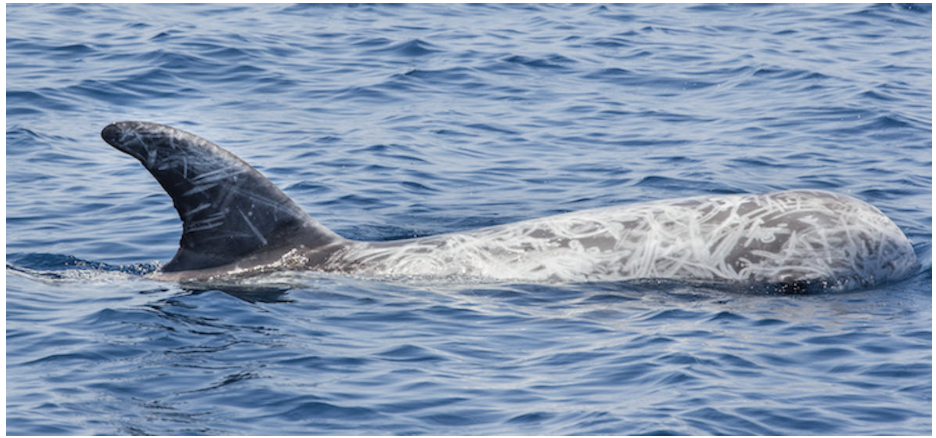
\includegraphics[width = 0.8\linewidth]{images/paper10/Risso.png}
    \centering
    \caption{Risso’s dolphins Grampus Griseus}
    \label{fig:Risso}
\end{figure}